\documentclass[a4paper,11pt]{article}


\usepackage{geometry}
\geometry{
 a4paper,
 left=30mm,
 top=30mm,
}
\usepackage[utf8]{inputenc}

\usepackage{graphicx}
\usepackage[english]{babel}
\usepackage{color}
\usepackage[dvipsnames]{xcolor}
\usepackage[colorlinks=true,urlcolor=blue,citecolor=black]{hyperref}
\usepackage{url}
%\urlstyle{same}
%\urlstyle{rm}
\urlstyle{sf}
%\urlstyle{tt}
\usepackage[font=footnotesize,labelfont=bf]{caption}
\usepackage[labelfont=it,textfont={it},singlelinecheck=on,justification=centering]{caption}
%full name for appendix
\usepackage[title]{appendix}
\usepackage{float}
\setlength{\parindent}{2em}
\usepackage{parskip}
%for code
\usepackage{listings}
%for math
\usepackage{amsmath}
\usepackage{pdfpages}
\linespread{1.1}
\setlength{\emergencystretch}{3em}

\usepackage{ifxetex,ifluatex}
\usepackage{etoolbox}
\usepackage{tikz}

\usepackage{framed}

%water mark
\usepackage{eso-pic}

\newcommand{\watermark}[3]{\AddToShipoutPictureBG{
	\parbox[b][\paperheight]{\paperwidth}{
		\vfill%
		\centering%
	\tikz[remember picture, overlay]%
	  \node [rotate = #1, scale = #2] at (current page.center)%
	      {\textcolor{gray!80!cyan!30}{#3}};
	  \vfill}}}
\usepackage{blindtext}
%water mark end


% conditional for xetex or luatex
\newif\ifxetexorluatex
\ifxetex
  \xetexorluatextrue
\else
  \ifluatex
    \xetexorluatextrue
  \else
    \xetexorluatexfalse
  \fi
\fi
%
\ifxetexorluatex%
  \usepackage{fontspec}
  \usepackage{libertine} % or use \setmainfont to choose any font on your system
  \newfontfamily\quotefont[Ligatures=TeX]{Linux Libertine O} % selects Libertine as the quote font
\else
  \usepackage[utf8]{inputenc}
  \usepackage[T1]{fontenc}
  \usepackage{libertine} % or any other font package
  \newcommand*\quotefont{\fontfamily{LinuxLibertineT-LF}} % selects Libertine as the quote font
\fi

\newcommand*\quotesize{60} % if quote size changes, need a way to make shifts relative
% Make commands for the quotes
\newcommand*{\openquote}
   {\tikz[remember picture,overlay,xshift=-4ex,yshift=-2.5ex]
   \node (OQ) {\quotefont\fontsize{\quotesize}{\quotesize}\selectfont``};\kern0pt}

\newcommand*{\closequote}[1]
  {\tikz[remember picture,overlay,xshift=4ex,yshift={#1}]
   \node (CQ) {\quotefont\fontsize{\quotesize}{\quotesize}\selectfont''};}

% select a colour for the shading
\definecolor{mygray}{gray}{0.95}
\colorlet{shadecolor}{mygray}

\newcommand*\shadedauthorformat{\emph} % define format for the author argument

% Now a command to allow left, right and centre alignment of the author
\newcommand*\authoralign[1]{%
  \if#1l
    \def\authorfill{}\def\quotefill{\hfill}
  \else
    \if#1r
      \def\authorfill{\hfill}\def\quotefill{}
    \else
      \if#1c
        \gdef\authorfill{\hfill}\def\quotefill{\hfill}
      \else\typeout{Invalid option}
      \fi
    \fi
  \fi}
% wrap everything in its own environment which takes one argument (author) and one optional argument
% specifying the alignment [l, r or c]
%
\newenvironment{shadequote}[2][l]%
{\authoralign{#1}
\ifblank{#2}
   {\def\shadequoteauthor{}\def\yshift{-2ex}\def\quotefill{\hfill}}
   {\def\shadequoteauthor{\par\authorfill\shadedauthorformat{#2}}\def\yshift{2ex}}
\begin{snugshade}\begin{quote}\openquote}
{\shadequoteauthor\quotefill\closequote{\yshift}\end{quote}\end{snugshade}}


\usepackage{listings}
\lstdefinestyle{myListStyle}{
  numbers=left,
  stepnumber=1,
  numbersep=10pt,
  tabsize=4,
  showspaces=false,
  showstringspaces=false
}

%opening
\title{\LARGE The Qitmeer White Paper:\\
	\Large The guardian of trust. The core network of the Halalchain}
\author{
	Qitmeer team\\
		\small\href{mailto:paper@qitmeer.io}
			{\nolinkurl{paper@qitmeer.io}}
	}
\date{\today\\\small Version 0.1}
\begin{document}

%% Cover end
\clearpage
\pagestyle{plain}

\maketitle

%\watermark{60}{10}{qitmeer.io}

\begin{abstract}

	Bitcoin was born with revolution, and it opened a new world that currency issuance becomes open and fair by a cryptography-based decentralized payment network. Further on, the underlying ledger mechanism of Bitcoin, i.e. blockchain, was found capable of playing a significant role in the financial field due to its temper-resistance. Islamic finance, as an essential part of world finance, also needing reshaping by blockchain. 

	With the arrival of 10-years birth of bitcoin, the blockchain infrastructure is 	facing various challenges from technical aspects. HLC considers openness, 	fairness, fault tolerance, scalability are the core metrics to asset a promising 	blockchain paradigm, and a blockchain system achieved a right balance among these metrics is deemed to satisfy Classical Blockchain Setting. 

	HLC develops a hybrid consensus that incorporates two BlockDAG protocols SPECTRE and GhostDAG. SPECTRE is extremely fast in confirmation, which is critical in a payment network. GhostDAG could provide transactional linearly ordering, which is the building block of reward mechanism. Both protocols are compliance with Classical Blockchain Setting - they could enter and leave network freely by Proof-of-Work, and the collaboration model of DAG ledger guarantees that miners gain rewards consistent with their devotion, 50\% faulty tolerance as secure as bitcoin, robust scalability that is only subject to physical network limit. The mining algorithm is also a vital source of fairness other than consensus algorithm per se. Cuckoo Ring is a graph theory based proof-of-work mining algorithm and is practically ASIC resistant due to memory hard calculation.
	
	HLC empowers UTXO model to achieve high available value storage and transfer network dedicated to Islamic finance. HLC's specific token issuance framework has considerably solved two main problems in terms of  Islamic finance being blockchain reshaped.  First, fundamental value support of issued tokens; second, Islamic Law Compliance.
	
	HLC devises a system of specifications and protocols to embrace the whole Isamlic financial ecosystem. Any third party could implement their own wallet, miner and mining pools by following this system. HLC integrates a robust cross-chain framework to interact with various cryptocurrencies; also, the reliable interoperability could offer off-chain smart contract support.

\end{abstract}

\section{Introduction}

\subsection{Background}
Trust is the cornerstone of finance. In traditional approaches, multiple unacquainted parties require a trustable third party to guarantee the security of transactions. However, this third party is centralized and subject to single point failure and unlikely to guarantee its honesty. 

Bitcoin is an open P2P network, that is to say, no centralized server exists, and each node can join or leave the network freely. The calculation-heavy but validation-easy Proof-of-Work consensus is designed to ensure nodes gain rewards relative to their contribution to the network's running and security, which is supposed to be fair — Bitcoin's disruption to drives tons of researches on its working mechanism. Bitcoin has a hash-list-like ledger to guarantee tamper resistance, further on the concept 'BlockChain' is introduced to represent this mechanism and commonly accepted. Owing to trustlessness and tamper resistance, more and more applications of blockchain occur in the financial field. Blockchain is reshaping finance.

However, with the arrival of 10-years birth of bitcoin, the blockchain infrastructure is facing various challenges from technical aspects and has been deviating its original intention. Bitcoin is no longer decentralized, the top 5 mining pool has controlled majority hash power and would be easy to carry on an attack if they found a reason to. Miners have to join mining pools since the opportunity cost is much higher than their contribution; in other words, Bitcoin is not fair any more. Bitcoin does not scale, seven transactions per second throughput, one hour confirmation time, high cost of the transaction fee, far from promising as a global payment network.

Bitcoin needs reform to return its original intention. Countless solutions arise and claim themselves having solved all these problems. However, few achieved indeed, just trading off one metric with another, e.g. sacrifice decentralization, which is a core source of security, for scalability. So, what the original intention of bitcoin truly is, Qitmeer has its definition and names it as Classical Blockchain Setting, it is also the design philosophy of Quitmeer.

\subsection{Classical Blockchain Setting}
Too many blockchain mutants and each has its definition of blockchain. Quitmeer respects bitcoin's vision, Qitmeer deems it is composed of 4 components and names it as Classical Blockchain Setting.

\subsubsection{Open}
Openness is the critical difference between permissioned and permissionless blockchain, so every node should join and leave the network freely. 

\subsubsection*{Predefined special roles}
An open network allows different role, in the bitcoin network, nodes could choose to be an SPV node, full node or miner with freedom, so from the protocol's aspect, bitcoin is open. Whereas, in Delegated Proof-of-Work, the block producers are voted outside of the chain and predefined as configuration, apparently not open enough.

\subsubsection*{Practically close}
Though bitcoin is open according to the protocol, it is close in practical. Miners are no longer independent and have to join mining pools, and this trend is getting worse. 


\subsubsection{Fair}
Fairness means that the rewards should be consistent with the contribution; in other words, Incentive-Compatible.

\subsubsection*{Opportunity Cost}
The expectation of rewards between standalone mining and pool mining is equal in terms of probability. The point is, their opportunity cost is considerably high - either mine a block to get a dramatically high reward or wait a long time without any return. So, they have to turn to the mining pool to have a stable incentive. 

\subsubsection*{Cost Efficiency}
It is mainly referring to mining cost. Mining cost mainly includes the electricity price and mining efficiency, and the latter is much more critical due to ASIC. ASIC is customized to direct a specific mining algorithm, so the mining efficiency per unit of cost is much higher than generalized computers. For instance, the hash rate per dollar for AntMiner S9 is about 20000 times greater than for GTX570; it is nearly impossible for a personal computer to win the hash rate competition.

\subsubsection{Secure}
The security is how robust the network is to sustain the attack, mainly referring to overrun a confirmed transaction.

\subsubsection*{Decentralization}
Decentralization is the most significant difference for bitcoin to be compared with traditional payment network. Decentralization could avoid single point failure; also, it is almost impossible to collude with the majority of all nodes in a fully decentralized network.
\subsubsection*{Fault Tolerance}
The network should be resilient to a certain proportion of misfunctioning resources, and  Tolerance is the upper bound of the percentage. In a decentralized network, 50\% fault tolerance is the ideal case according to the majority law.

\subsubsection{Scalable}
A network that can offer relatively stable services with its scale increasing is considered scalable. Blockchain network includes the following services:
\subsubsection*{Throughput}
How many transactions per second when network is scaling. Bitcoin's throughput is upper bound to 7 TPS, no matter how many nodes are there in the network.
\subsubsection*{Confirmation}
How long does the recipient to wait until his transaction is believed unlikely to be overrun? The waiting time should not increase with networking scaling.
\subsubsection*{Cost}
The main component of cost is transaction fee, and it should be reasonable, it would make payment impractical if too high, whereas be subject to sybli attack if too low. With the mining difficulty increasing, Bitcoin transacation fee is getting higher and higher, and it won't be suitable to serve as a global payment network as it aimed to, up to the time this paper finished, the average price of bitcoin is rough 2\$ . [https://bitcoinfees.info/]

\subsection{Specification}
Qitmeer's specification is designed to abide by Classical Blockchain Setting
\subsubsection{Openess}
Qitmeer is an open network; it uses proof-of-work to join the network freely and use BlockDAG protocol to avoid the risk of mining pools centralization.
\subsubsection*{Proof of Work}
Proof-of-Work is the openest way so far to join a blockchain network because the only resource required to contribute to is electricity, which every node has owned. Besides, this resource is physical; in other words, it is non-duplicatable. 
\subsubsection*{No Predefined Nodes}
 Quitmeer doesn't have predefined sepcial nodes , i.e. super nodes.
\subsubsection{Fairness}
BlockDAG is fair because it is a collaboration model other the competition model of blockchain.
\subsubsection*{Mining Pool Resistance}
Mining pools centralization is the consequence of high opportunity cost, which is the consequence of the competition model. Qitmeer's BlockDAG-based protocol SPECTRE is a collaboration model, the opportunity cost of standalone mining is equal to that of pool mining, so it will not be necessary to join a mining pool, which would lead to the risk of centralization.
\subsubsection*{Anti-ASIC Mining Algorithm}
Cuckoo Cycle is a graph-theoretic proof-of-work algorithm and prevails for ASIC resistance. Qitmeer employs this algorithm to guarantee that no one has too much mining efficiency advantage.
\subsubsection{Security}
Security is the first code in Quitmeer, and it is a fully decentralized and 50\% fault tolerant, which is the most stringent criteria; thus, there is no security sacrifice for other metrics. 
\subsubsection*{Fully Decentralization}
All the nodes in the Qitmeer's network are peer nodes and can participate in consensus.
\subsubsection*{50\% Faulty Tolerance}
The malicious adversary has to posses 50\% hash power to control the network. Either in SPECTRE or GhostDAG, the fault tolerance is irrelevant with the throughput, whereas the security is inversely propagational to throughput in bitcoin.

\subsubsection{Scalability}

Qitmeer's hybrid BlockDAG protocols scales, fast confirmation, high throughput, low transaction fee, all these features ensure Qitmeer will be running stably in a considerable long time.
\subsubsection*{Fast Confirmation}
SPECTRE is a speedy confirmation BlcokDAG protocol, and Qitmeer uses as its consensus algorithm.
\subsubsection*{High Throughput}
SPECTRE is a BlcokDAG protocol, and the throughput could grow up to the network's physical metrics, such as network bandwidth or propagation delay.
\subsubsection*{Low Cost}
Strictly speaking, the cost is not scaling since the transaction fee is increasing slightly with the network growing. However, the average cost will keep relatively low and acceptable for a long time. So, from the reasonableness aspect, the cost scales.

\section{Qitmeer Token Design}

The HLC public chain is a powerful innovative technology that has the potential to transform the global Islamic financial services industry. it is a distributed database of records or public ledger of all transactions or digital events that have been executed and shared by corporate entities. HLC technology is cryptographically authenticated. It is developed to provide an alternative secure approach to exchange value without the involvement of third party. The technology enables simplification and brings in greater security, scaleability, speed, and reliability. The results is reduced costs and improved efficiency. 

\subsection{Overview}

The $\texttt{OP\_TOKEN}$ is inspired by Color coin idea, which represents and manages real world assets on top of the Bitcoin by using $\texttt{OP\_RETURN}$, and the OP\_GROUP, a referenced implementation of issuring assets designed by Andrew Stone.

The OP\_TOKEN fit various practical scenarios with unique features like asset compliable and value relevent. There are some related concepts in the details below:  

\subsubsection{UTXO}

UTXO represents Unspent Transaction Output. A transaction has multiple sources and destinations, which we call them inputs and outputs. There are no accounts in HLC. What users have and spend are a bunch of unspent transaction ouputs and we could get balance by summing up them. 

\begin{figure}[hbt]
	\centerline{%
	   \resizebox{0.8\textwidth}{!}{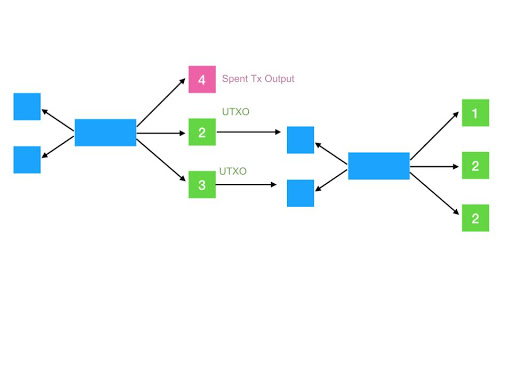
\includegraphics{figures/utxo-1.jpg}}%
	}
\caption{utxo model}
\end{figure}


The first transaction tx1 has 3 outputs and the first output of them is spent, so  tx1 has 2+3=5 coins balance. 

The second transaction tx2 spends the 2 UTXOs of tx1 and pays to 3 addresses and creates 3 new UTXOs. 

Note: now the old UTXOs (of tx1) are no longer UTXO so cannot be spent later.  

\subsubsection{Script system}

The mechanism behind how users spend their UTXOs is to execute a special script. The output stores a half of the script and we have to present the other half and combine both to verify if we could spend the money. The former half is called locking script, like a locked treasure box, and the latter is unlocking script, like the only key to the box.

Let's take a look at the typical instance of  Pay-2-Public-Key-Hash(P2PKH)

Locking Script in UTXO:

\begin{lstlisting}
OP_DUP OP_HASH160 <PUBLIC_KEY> OP_EQUALVERIFY OP_CHECKSIG
\end{lstlisting}

Unlocking Script in a newly created transaction:

<Signature><PublicKey>

Combine unlocking script with locking script:

<Signature><PublicKey> OP\_DUP OP\_HASH160 <PUBLIC\_KEY> OP\_EQUALVERIFY OP\_CHECKSIG

This whole script consists two steps
1. <PublicKey>  OP\_HASH160 <PUBLIC\_KEY> OP\_EQUALVERIFY
	To very if the public key in the unlocking script matches that in the locking script.
2.  <Signature><PublicKey> OP\_CHECKSIG
	To check if the signature is valid.


\subsubsection{Color coin and USDT}

Color coin is a method to represent assets on top of the blockchain, so it can leverage the tamper-proof capibility of blockchain. It uses tx-script operation $\texttt{OP\_RETURN}$ to interupt script execution early, so we can add information of the assets after it without violating the script validation.

Locking Script:
\begin{lstlisting}
OP_RETURN <DATA>
\end{lstlisting}

The stable coin Tether (USDT) also uses OP\_RETURN based omni layer protocol to define the asset on the bitcoin. 

Here is a typical USDT transacation and details of its protocol design


\lstset{basicstyle=\tiny,style=myListStyle}
\begin{lstlisting}
OP_RETURN 6f6d6e69000000000000001f00000015c9054900
\end{lstlisting}


\begin{figure}[hbt]
	\centerline{%
	   \resizebox{0.8\textwidth}{!}{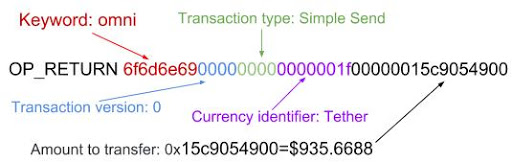
\includegraphics{figures/usdt.jpg}}%
	}
\caption{usdt}
\end{figure}


%[ref][https://www.blockchain.com/btc/tx/efc50d9e1f23e687e304cfca4ef2c5412b67d5737888ff80a0cbb6853cd865c]



\subsubsection{OP\_GROUP}
The OP\_RETURN scheme is more suitable to apply on mature blockchain since it doesn't change the underlying blockchain protocol and won't risk forking. However, the weakness  is that miners cannot verify its protocol so there would be some security risks.

OP\_GROUP is a proposal of assets issuance  on Bitcoin Cash (BCH) from Bitcoin Unlimited (BU) and has been approved by BU. OP\_GROUP supports token issuance, tranfer, destroy, etc. Since OP\_GROUP is an extention to BCH script sytem,  it is part of BCH protocol and can be verified by miners, which is more reliable.

The basic “colored” pay 2 public key hash script would be like: 

\lstset{basicstyle=\tiny,style=myListStyle}
\begin{lstlisting}
OP_DATA(group address)  
OP_GROUP  
OP_DROP  
OP_DUP  
OP_HASH160  
OP_DATA(pubkeyhash)  
OP_EQUALVERIFY  
OP_CHECKSIG
\end{lstlisting}

The main difference is simple, just adding a group address to distiguish different groups, and other operations, such as create and destroy assets, are similar.

% [ref]https://medium.com/@g.andrew.stone/bitcoin-scripting-applications-representative-tokens-ece42de81285

\subsection{OP\_TOKEN Design}

\subsubsection{Overview}

There is a special token named LICENSE in OP\_TOKEN. Licenses are held by renowned expects or organizations with public credibility. Any entitity planing to issue a token needs to be warranted a license. Since license is also a token, it is able to be transfered between peers. However, license transfer can be tracked through transaction history, so the originator would be very cautious in case transfering to a wrong hand.

\subsubsection{Issuance of License}

Licenses are all generated in genesis block and distribted to 100 preserved committe members. One smallest unit of HLC (SAND) represents a license,  one block has 100 HLC,  1 HLC= 10\^8 SAND , so we have 10 \^10 license in total, which is sufficient for asset issuance.


\lstset{basicstyle=\tiny,style=myListStyle}
\begin{lstlisting}
INPUTS:
	INPUT:
		PREVIOUS_OUTPUT: # (COINBASE of GENESIS)
		SCRIPT: "DUP HASH160 [GENESIS_HASH] EQUALVERIFY CHECKSIG"
		VALUE: 10000000000 (10 billion)
		SCRIPT: "[SIG] [GENESIS_PK]"
OUTPUTS:
	OUTPUT:
		SCRIPT: "[LICENSE_HASH] TOKEN DROP DUP HASH160 [COMMITTEE_1_HASH] EQUALVERIFY CHECKSIG"
		VALUE: 100000000 (100 million)
	# ... ... (COMMITTEE 2~99)
	OUTPUT:
		SCRIPT: "[LICENSE_HASH] TOKEN DROP DUP HASH160 [COMMITTEE_100_HASH] EQUALVERIFY CHECKSIG"
		VALUE:100000000#(100 million)
	OUTPUT:
		SCRIPT: "RETURN [DATA]" 
		VALUE: 0
\end{lstlisting}


\subsubsection{Warrant a license}

The individual and corporate entities/companies must be warranted a license to issue assets. These companies can request license from any committee member. Once the license is granted and approved, it would receive a special token transfer from the commitee member and the token is the license.

\lstset{basicstyle=\tiny,style=myListStyle}
\begin{lstlisting}
INPUTS:
	- INPUT:
		PREVIOUS_OUTPUT:
			SCRIPT: "[LICENSE_HASH] TOKEN DROP DUP HASH160 [COMMITTE_HASH] EQUALVERIFY CHECKSIG"
			VALUE: 100000000
		SCRIPT: "[SIG] [COMMITTE_PK]"
OUTPUTS:
	- OUTPUT:
		SCRIPT: "[LICENSE_HASH] TOKEN DROP DUP HASH160 [ISSUER_HASH] EQUALVERIFY CHECKSIG"
		VALUE: 1
	- OUTPUT:
		SCRIPT: "[LICENSE_HASH] TOKEN DROP DUP HASH160 [COMMITTE_HASH] EQUALVERIFY CHECKSIG"
		VALUE: 99999999
	- OUTPUT:
		SCRIPT: "RETURN [DATA]" 
		VALUE: 0
\end{lstlisting}

\subsubsection{Issuance of assets}
Once warranted a license, organizations are able to issue assets. Assets cannot be built from the air, they required equal amount smallest unit (sand) of HLC to be converted. This process is called as "token mint". it is like to mint a gold coin requires the same weight of gold sands, tokens need same amount of HLC sands. The advantage is not only that the token has a value support by underlying currency but also that all tokens and HLC are invovled in the same ecosytem, which would improve the liquidity and make whole network healthier.

\lstset{basicstyle=\tiny,style=myListStyle}
\begin{lstlisting}
INPUTS:
	- INPUT:
		PREVIOUS_OUTPUT: #(1 LICENSE)
			SCRIPT: "[LICENSE_HASH] TOKEN DROP DUP HASH160 [ISSUER_HASH] EQUALVERIFY CHECKSIG"
			VALUE: 1
		SCRIPT: "[SIG] [LICENSE_PK]"
	- INPUT:
		PREVIOUS_OUTPUT: #(1 HLC)
			SCRIPT "DUP HASH160 [COIN_HASH] EQUALVERIFY CHECKSIG"
			VALUE: 100000000
		SCRIPT "[SIG] [COIN_PK]"
OUTPUTS:
	- OUTPUT:
		SCRIPT: "[LICENSE_HASH] TOKEN DROP DUP HASH160 [ISSUER_HASH] EQUALVERIFY CHECKSIG"
		VALUE: 1
	- OUTPUT:
		SCRIPT: "[TOKEN_HASH] TOKEN DROP DUP HASH160 [PK_HASH] EQUALVERIFY CHECKSIG"
		VALUE: 100000000
	- OUTPUT:
		SCRIPT: "RETURN [DATA]"
		VALUE: 0
\end{lstlisting}

\subsubsection{Transfer of the Assets}

Assets can be transfered between parties. Moreover, we could transfer mulitple assets within one transaction. The transaction needs to ensure the  input sum of each asset equals the output sum of each asset. 

\lstset{basicstyle=\tiny,style=myListStyle}
\begin{lstlisting}
INPUTS:
	- INPUT:
		PREVIOUS_OUTPUT:
			SCRIPT: "[RMB] TOKEN DROP DUP HASH160 [ACLICE_PKHASH] EQUALVERIFY CHECKSIG"
			VALUE: 100
		SCRIPT: "[ALICE_SIG] 0X83 [ACLIE_PUBKEY]"
	- INPUT:
		PREVIOUS_OUTPUT:
			SCRIPT: "[USD] TOKEN DROP DUP HASH160 [BOB_PKHASH] EQUALVERIFY CHECKSIG"
			VALUE: 20
		SCRIPT: "[BOB_SIG] 0X83 [BOB_PUBKEY]"
OUTPUTS:
	- OUTPUT:
		SCRIPT: "[USD] TOKEN DROP DUP HASH160 [ALICE_PKHASH] CHECKSIG"
		VALUE: 20
	- OUTPUT:
		SCRIPT: "[RMB] TOKEN DROP DUP HASH160 [BOB_PKHASH] CHECKIG"
		VALUE: 100
\end{lstlisting}


\subsubsection{Unmint Token}

In addition to mint token, the Token can unmint. as the Token  we cannot build from nothing, we cannot destroy tokens into ashes, instead, we melt  tokens into HLC. Also, tokens can be melt into the same amount of HLC sands. So, tokens have minimum value sustain. 

However, HLC encourages token holders to increase their token values rather than unminting them. But there are some scenarios to make unminting practical, such as stable coins. So, HLC only allow the token issuer to umint tokens.

\lstset{basicstyle=\tiny,style=myListStyle}
\begin{lstlisting}
INPUTS:
	- INPUT:
		PREVIOUS_OUTPUT:
			SCRIPT: "[TOKENHASH] TOKEN DROP DUP HASH160 [ISSUER_HASH] EQUALVERIFY CHECKSIG"
			VALUE: 100
		SCRIPT: "[SIG] [ISSUER_PUBKEY]"
OUTPUTS:
	- OUTPUT:
		SCRIPT: "DUP HASH160 [COIN_HASH] EQUALVERIFY CHECKSIG"
		VALUE: 100
	- OUTPUT:
		SCRIPT: "RETURN [DATA]"
		VALUE: 0
\end{lstlisting}


\section{Consensus Protocol}


\subsection{Introduction of DAG Technology}

Block DAG, as the name implies, is a DAG paradigm of ledger in which each node
is a block. In fact, each node in the ledger can either be a block or a
transaction, because a transaction can also be regarded as a block which
contains only one transaction.

Block DAG tries to solve the scalability problem of blockchain on protocol
level. Although scalability limits can be broken through in many ways, such as
raising up processing speeds, disk I/O and so on, a major barrier lies in
blockchain paradigm itself: the orphan rate. Orphans are blocks that are created
outside the longest chain due to unavoidable network propagation delays. In
blockchain paradigm, orphan blocks waste network bandwidth and do not contribute
to throughput. What's worse, the two intuitive ways to improve scalability, which
are to increase the block rate and the block size, both increase the orphan
rate. The higher the orphan rate is, the less secure the chain
is\cite{Yonatan-high-rate-bitcoin}\cite{bitcoin-backbone}\cite{asynchronous}.

In other words, Bitcoin sacrifices scalability for security to achieve low
orphan rate as possible.

Block DAG tries to solve the tradeoff by allowing blocks to reference multiple
predecessors instead of a single parent. Compared with other schemes such as
sharding and layering which also try to solve the scalability problem, the Block
DAG way is simple and intuitive. It's just a structural alternative to
blockchain. The other aspects can be the same as Bitcoin. Nodes can still
participate freely to realize complete decentralization.  Security can still be
guaranteed as long as more than 50\% of the computing power are honest.

\begin{figure}[hbt]
	\centerline{%
	   \resizebox{0.8\textwidth}{!}{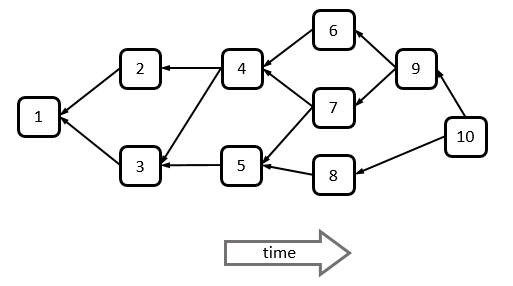
\includegraphics{figures/DAG.png}}%
	}
\caption{DAG}
\end{figure}

Of course, a DAG ledger may contain conflicting transactions since different
chains are incorporated. Therefore, new consensus protocols are necessary to
provide high scalability without losing security.

\subsection{Consensus}
HLC adopts Hybrid consensus that combines SPECTRE and GHOSTDAG (Phantom) in order to achieve fast confirmation and high throughput.


\subsubsection{SPECTRE}
SPECTRE is a block-DAG based protocol that achieves fast comfirmation and high
throughput with 50\% attack resilience. SPECTRE guarantees safety, which means a
transaction is unlikely to be reversed once it is accepted. Also, SPECTRE guarantees fast confirmations for honest users rather than all users, so it is deemed as weak liveness.

There is a trade off between liveness and fast confirmation, SPECTRE prioritize
the latter since weak liveness only affects malicious users. SPECTRE is built
for payment model. Only malicious users launch douple spends, so only their
transactions are likely to be delayed indefinitely.

SPECTRE is built for stateless transaction model, so there is no need to gain a
total ordering over all the blocks. Only when there're two blocks conflicting
that a pairwise ordering is needed.

SPECTRE employs a voting algorithm to decide which block wins when two blocks
conflict. Suppose block $x$ has a conflicting transaction with another
transaction in block $y$, and also suppose that block $z$ is voting on them with
the following rules:


\begin{enumerate}
	\item If $z$ is in $x$'s future but not in $y$'s future, $z$ votes for
		$x$ in favor of $y$, denoted as $x \prec y$, and vice versa.
	\item If both $x$ and $y$ are in the past of $z$, then $z$ follows the majority votes in its past.
	\item If neither $x$ nor $y$ is in the past of $z$, then $z$ follows the majority votes in its future.
	\item Both $x$ and $y$ vote for themselves unless one is in the past of
		the other.
\end{enumerate}


Here's an example of how a new block (number 12 in the figure below) votes:

\begin{figure}[h]
	\centerline{%
	   \resizebox{0.8\textwidth}{!}{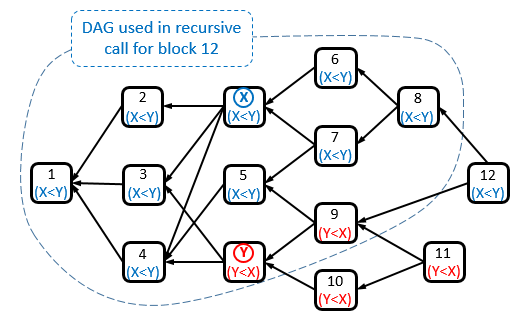
\includegraphics{figures/SPECTRE}}%
	}
\caption{An example of the voting procedure in the DAG for blocks $x$ and $y$ in SPECTRE}
\end{figure}

According to rule 4, block $x$ votes for $x \prec y$, block $y$ votes for $y
\prec x$.

According to rule 1, blocks 6, 7 and 8 vote for $x \prec y$, blocks 9, 10 and 11
vote for $y \prec x$.

According to rule 2, block 12 votes according to its past. Since not all blocks
of its past have voted, we change global view to block 12's local view, which
means block 10 and 11 are excluded.

According to rule 3, block 5 votes for $x \prec y$, since the majority of its
future vote in favor of $x$ over $y$ (blocks 7, 8 versus block 9). Note that the
current view is block 12's local view and block 11 is exculded, so we cannot
take its vote.

Also according to rule 3, blocks 1\textasciitilde4 vote for $x \prec y$.

Now all the blocks in block 12's past have voted. Block $x$ gets 10 votes. Block
$y$ gets 2 votes. Block 12 follows the majority and votes for $x \prec y$ thus.

\subsubsection{PHANTOM}

Since HLC technology is based on transaction model, in most cases it is
sufficient to provide only partial ordering or pairwise ordering for blocks in
the ledger. However, sometimes we may still need to obtain a total (linear)
ordering of all the blocks, especially when we want to reward blocks based on
their ordering. 

Obtaining total ordering for a DAG ledger is not so intuitive as it is for
blockchains since a DAG ledger contains forks, which are caused by network
propagation delay, concurrent block creations, faulty miners, and so on.
Therefore, as a supplement to the consensus protocol of HLC, we use PHANTOM to
obtain the total ordering to reward blocks which appears earlier in the
ordering.

In addition to total ordering, PHANTOM also provides strong liveness guarantee
to make the consensus protocol more robust, which means both honest blocks and
malicious blocks can be confirmed within definite time, though it may take a
long time to confirm malicious blocks.

Suppose that the maximal limits of network propagation delay and block creation
rate are constant. It is intuitive that if nodes behave honestly, they will form
a sub graph where each block has at most a constant number of forks. We denote
this constant number as $k$. $k$ can be caculated from propagation time and
block creation rate. The sub graph is denoted as a $k$-cluter. The biggest
$k$-cluster is called a blue set. Those blocks outside the blue set are called
red set.

If we can traverse from block $x$ to block $y$ by following the parent
references within each block, then we say that there's a partial order between
$x$ and $y$, and $y$ is prior to $x$. For example in the following figure, we
can traverse from block J to A through B, so there's a partial order between A
and J, and A is prior to J. Note not all blocks have partial orders with other
blocks. For example, there're no partial orders between B, C and D. We call the
block set where no partial order exists an anticone. The size of any anticone in
a $k$-cluster is at most $k$.

\begin{figure}[h]
	\centerline{%
	   \resizebox{0.8\textwidth}{!}{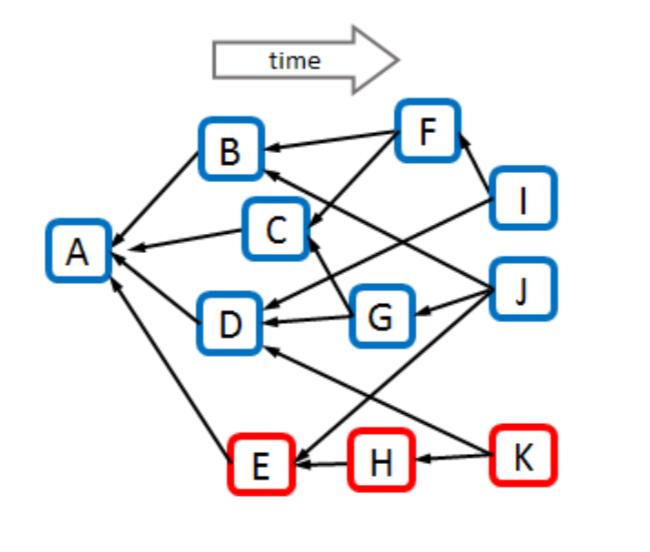
\includegraphics{figures/PHANTOM}}%
	}
\caption{PHANTOM}
\end{figure}


PHANTOM orders the DAG ledger in a way that favours blue blocks and penalizes
red ones. We determine the order between blue blocks according to their partial
orders and some topological sort. Then, for any blue block $B$, add to the order
just before $B$ all of the red blocks in $past(B)$ that weren’t added to the
order yet; these red blocks too should be added in a topological manner. Notice
that for any blue block $B$, the order on blocks in $past(B)$ should remain the
same if we remove from the DAG blocks in $future(B)$. This can be implemented,
for instance, using a priority queue that pops out blocks according to the size
of their past set.

An example of the output order of the PHANTOM procedure on the small DAG ledger
from the figure above is: $(A,D,C,G,B,F,I,E,J,H,K)$. Unfortunately, finding the
maximum $k$-cluster is NP hard, so PHANTOM is therefore of less practical use
for an ever-growing DAG ledger and may causes long confirmation times.
Therefore, we use PHANTOM only to implement the reward mechanism of HLC, since
it should be acceptable for a miner to wait for a while to get his or her mining
reward. The confirmation time for a transaction to be accepted is still defined
in the SPECTRE way.

\subsubsection{Cuckoo-Cycle-PoW}

Proof-of-Work(PoW) is used to confirm transactions and produces new blocks, therefore it is a very important engine in PoW cryptocurrencies. PoW must not enable a participant to have a significant advantage over another participant. That is why Satoshi said: "Proof-of-work is essentially one-CPU-one-vote."

However, most widely used proof-of-work algorithms, such as SHA-256, Blake2b, Scrypt, are more efficient on ASIC devices when compared to CPUs and GPUs. This can lead to ASIC owners posses a much larger voting power than CPU and GPU owners. It violates the “one-CPU-one-vote” principle.

We introduce Cuckoo-Cycle-PoW ,a graph-theoretic proof-of-work algorithm. It is ASIC resistant.

Cuckoo-Cycle-PoW is designed to find certain subgraphs in large pseudo-random graphs. This algorithm that we hope turns out to be ASIC resistant. It utilizes almost all parts of commodity hardware (GPUs).

The Cuckoo Cycle POW is the work of John Tromp, it is designed to find certain subgraphs in large pseudo-random graphs. In particular, Search for cycles of specified length L in a bipartite graph with M edges of N nodes. If a cycle is found and the hash difficulty is less than the target difficulty, the cuckoo cycle PoW is completed.


\textbf{Overall flow}

\begin{enumerate}
	
\item Outer loop

\begin{enumerate}
	\item Build block Header with following values:
	
		\begin{itemize}
		\item Difficulty: Difficulty target for tx
		\item TxRoot: The merkle root of the tx tree
		\item Timestamp: A Unix time timestamp
		\item Nonce: A 64-bit (8-byte) field whose value is adjusted by miners
		\item ParentRoot: The merkle root of the previous parent blocks (the dag layer)
		\end{itemize}
	
	\item Set amount of the attempt time, currently configured at 60 seconds, for inner loop.
	\item Set the deadline is equal to the attempt time add the current unix timestamp.
	\item Inner loop
	
		\begin{enumerate}
			\item Check the header’s hash is the latest header’s hash and the current timestamp less than the deadline.
			\item Initialize cuckoo graph with some consensus values, such as edgebits(the size of the graph),proofSize(the length of the cycle)
			\item The Blake2b algorithm hashes the block header.
			\item Through the SIPHASH function to build nodes of graph, the block header’s hash and the nonce of inner loop as input parameters.
			\item Edge Trimming: It drastically reducing the number of edges our basic algorithm has to process.
			\item The finding cycle algorithm tries to find a solution (i.e. a cycle of length 42) within the generated graph.
			\item If the solution is found:
			
			\begin{enumerate}
				\item The Blake2b algorithm hashes the cycle nonces.
				\item The cycle nonces’s hash is compared to the current target difficulty.
			\end{enumerate}
		
			\item If the cycle nonces’s hash difficulty is greater than or equal to the target difficulty, the block is sent to the transaction pool, propagated amongst peers for validation, and work begins on the next block.
			\item If the cycle nonces’s hash difficulty is less than the target difficulty, the proof is thrown out and the inner loop continues.
		\end{enumerate}
		
\end{enumerate}

\end{enumerate}


\textbf{Edge(Node) generation}

For the sake of simplicity, we define 32 edges for the bipartite graph. We call the SIPHASH function twice to create two edge endpoints(U and V), with the first input value being 2 * nonce, and the second 2 * nonce+1. The key for this function is based on a hash of a block header.

\begin{equation}
{U = SIPHASH(headerHash, 2*nonce) \mod 31}
\end{equation}
\begin{equation}
{V = SIPHASH(headerHash, 2*nonce+1) \mod 31}
\end{equation}

where,
\begin{equation}
0\leq\ {\bf nonce} \leq 31
\end{equation}it is any number between 0 and 31. Each nonce corresponds to two edge endpoints(U and V).

To throw 32 edges into a graph, randomly:

\begin{figure}[h]
	\centerline{%
		 \resizebox{0.8\textwidth}{!}{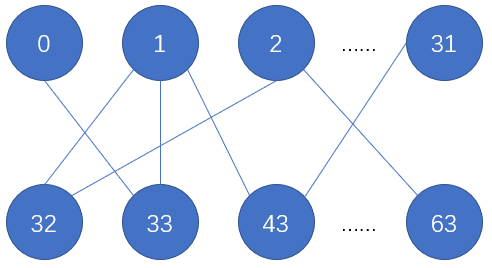
\includegraphics{figures/edge_generation}}%
	}
	\caption{Building Nodes.}
\end{figure}


\textbf{Edge Trimming}

There is a special edge in bipartite graph, which we call leaf edges. It can never be part of a cycle.
Leaf edges have a feature, the nodes it connects must have at least one node with the degree of the nodes being one.
By eliminating leaf edges in the bipartite graph, we can greatly reduce the complexity of the graph,
thus speeding up finding cycle from the bipartite graph.

\begin{figure}[h]
	\centerline{%
		 \resizebox{0.8\textwidth}{!}{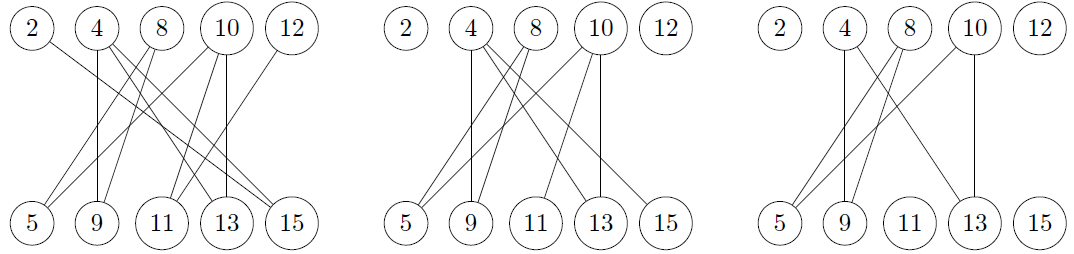
\includegraphics{figures/edge_trimming}}%
	}
	\caption{Trimming of edges which cannot be part of a cycle.}
\end{figure}

\begin{itemize}
	\item Step 1: node 0, node 3 and node 10 are one degree nodes, eliminating the edge (0,13), (6, 3) and the edge (10,9).
	\item Step 2: node 9 and node 13 are one degree nodes, eliminating the edge (8,9) and the edge (2,13).
	\item Step 3: node 8 is one degree nodes, eliminating the edge (8,11).
\end{itemize}


\textbf{Cycle detection}

After edge trimming, if a cycle of length L is found, we think we have found a solution to this problem.
we store the cycle edges in a set and put the nonce of the generated cycle in a set and
return as the result of cycle detection.


\textbf{Difficulty control}

The difficulty of finding a cycle in the graph is proportional to M/N. Here M stands for edges of the graph.
N stands for nodes of the graph. However, the difficulty of finding a cycle in the graph change is not smooth.
For crypto currencies, difficulty control must be scale in precisely controlled manner. The usual practice is
that the ratio of M/N remain fixed, such as M/N = 1/2.
The figure is probability trend of finding a cycle of length 42.

\begin{figure}[h]
	\centerline{%
		\resizebox{0.8\textwidth}{!}{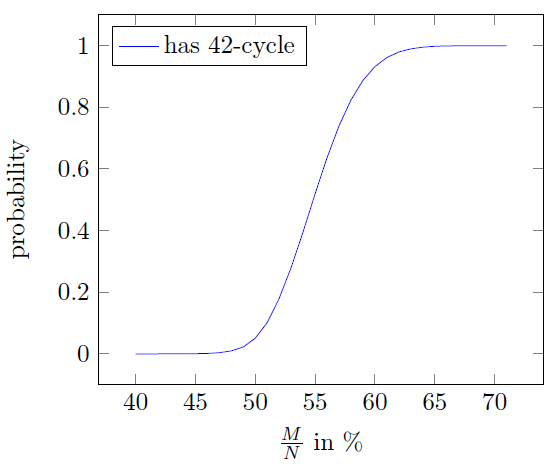
\includegraphics{figures/probability}}%
	}
	\caption{Probability trend.}
\end{figure}

Thus in the actual use, it also adds a hash difficulty control similar to Bitcoin. The digest of the cycle nonces is obtained by a hash function,
and then compared with the target difficulty.

\section{HLC Innovation}
\subsection{Both liveness and fast confirmation} 
SPECTRE is quite a fast comfirmation protocol for payment, with just one slight weakness - weak liveness. It affects only misfunctioning transactions and even would make them unconfirmed indefinitely. Although it won't affect honest nodes, it is more robust for all nodes to have strong liveness.

\subsection{Consensus algorithms efficiency} 

\subsection{Storage efficiency} 

\subsection{Transaction replication} 

\section{Award}

\subsection{CoinBase}

\subsection{Transaction Fee}

Miners are profitable and tend to pack the transaction with higher fees. This will result in high repetition rates of blocks. Repeated transactions will not contribute to the throughput. So we need to design an incentive mechanism to guide the miners, which makes them try not to pack duplicate transactions. Inclusive introduced a mechanism to split the transaction fee. In this way, if all the miners go to package a high-fee transaction, it may eventually cause the miner to only package the transaction with high transaction fee, but the income will decrease. Finally, through the game, everyone will randomly select the transaction from the memory pool to reach the Nash equilibrium. According to the data of the paper, the repetition rate can be controlled at around 30\%.

The trasaction halving scheme of Inclusive is complicated to implement, because the block confirmed number is not fixed. The block may be confirmed by the newly generated block at any time, so it is supposed to add a lot of control logic to implement this. Secondly, this design, in fact, it does not motivate users to quickly release blocks. Because whether it is released early or later, it can be divided into fees. In addition, it is unfair to simply randomly select transactions. If the probability how much the fees is random, the transaction will choose a low fee or even send a junk transaction, nor will it meet the need to quickly be confirmed by increasing the fee.

Therefore, HLC's plan, firstly, is to randomly select the desired transaction according to the weight of each transaction, so as to ensure that the user is willing to use the higher handling fee to attract the miners to pack the transaction, and the comprehensive income of the miner is also improved and they are more willing to mine. Secondly, the transaction fee can only be owned by the miners who originally packed the transaction. The order of the blocks in the transaction is determined by the PHANTOM protocol. This encourages the user to publish the block as early as possible.

In order to ensure the stability of the block order, the block reward needs to wait for 100 confirmed blocks to be spent.

\subsection{Cuckoo Cycle}
TODO[Jin, 1+ pages]: Introduction, 

\subsection{Confirmation time}
\subsubsection{Formal introduction}
TODO[Xiang, 2+ pages]
\subsubsection{Simulation Report}
TODO[Jin, 1+ pages]

\section{Ecosystem}
TODO[forchain]: Overview

\subsection{Mining Protocol}
\subsubsection{Proof-of-work Algorithm}

We hope to resist the centralization of mining power, and hope miner can utilizes almost all parts of commodity hardware (GPUs, CPUs).
Therefore, Qitmeer uses a Proof-Of-Work algorithm called Cuckoo Cycle\cite{cuckoocycle}, 
a memory-hard algorithm.This algorithm is designed to find certain subgraphs in large pseudo-random graphs. 
An introduction of Qitmeer proof-of-work can be found here.\cite{qitmeerpow} 

\subsubsection{Miner Capability}

At the moment, the fastest GPU miner implementation is HLC-Miner, which developed by the HLC developers. 
However, the HLC-Miner is still in the early stage of development, It's not a deeply optimized version. We hope 
that the community will finally create more optimised miners.

The HLC-Miner support parallel GPU. You can run multiple Nvidia GPUs and AMD GPUs mining in parallel.

Compatible GPU Hardware:

\begin{itemize}
\item Nvidia: GTX1060 GTX1070, GTX1070ti, GTX1080, GTX1080ti, GTX2070, GTX2080, GTX2080ti
\item AMD: RX570, RX580, Vega56, Vega64
\end{itemize}

In principle, as long as the graphics memory is greater than 5GB, the GPU miner can run.

The HLC-Miner support both solo mining and pool mining. 

\subsubsection*{Solo}
If you do decide to mine Qitmeer without joining a pool, these are the steps to achieve mining Qitmeer by yourself.

\begin{itemize}
\item You need to run a full node to validate transactions. First, install qitmeer\cite{qitmeer} with the complete blockchain downloaded. Qitmeer is a full node software program that fully validates transactions and blocks. 
\item Download and install the Qitmeer miner software like HLC-Miner. For a solo miner, the mining software connects to the blockchain full node (Qitmeer). The main job of the miner software is to create valid Proofs-of-Work and deliver the block to the rest of the Qitmeer network.
\item Finally, launch Qitmeer miner software and connect to Qitmeer network to start solo mining Qitmeer.
\end{itemize}

\subsubsection*{Pool}
Most mining pools support stratum protocol, so your miner program should be config this protocol. 
For example:

\emph{miner.exe -o stratum+tcp://serverIp:3177 -m YourWalletAddress.YourMachineId}

\subsubsection{Mining Pool Capability}
The Proof-Of-Work algorithm implementation in Qitmeer is perfect for a mining pool.


\subsection{Wallet Protocol}
TODO[Logan, 1+ pages]: Protocol, Interface, Specification

\subsection{Cross Chain}
TODO[forchain 1 page]: Overview

\subsubsection{UTXO interoperability}
TODO[Yi, 1+ page]:  mechanism

\subsubsection{Smartcontract interoperability}
TODO[Yi, 1+ page]: mechanism

\section{Future Work}
Undetermined [forchain] 



\clearpage
%\appendix
%\section{Appendix}
%\begin{appendices}
%\section{append A}

%Foo bar Foo bar Foo bar Foo bar Foo bar Foo bar Foo bar Foo bar Foo bar Foo bar

%\end{appendices}

%\bibliographystyle{plainnat}
%\bibliographystyle{unsrt,acm}
\bibliographystyle{unsrt}
\bibliography{hlc_whitepaper}

\end{document}

